\section{Einführung}
\label{sec:Introduction}


\subsection{Grundideen}
\label{subsec:basic-concepts}
\begin{frame}
	\frametitle{\insertsubsection}
	\begin{itemize}[<+->]
		\item Änderung der Variable hängt von Variable selbst ab

	\end{itemize}
\end{frame}


\subsection{Beispiele}
\label{subsec:examples}
\begin{frame}
	\frametitle{\insertsubsection}
	\begin{itemize}[<+->]
		\item Corona-Neu-Infizierungungen (Änderung) sind proportional zu der Anzahl der bereits infizierten Menschen
		\[\dot{N} = a N\]
		\item[$\Rightarrow$] Exponentielles Wachstum $N=N_0\exp(at)$
		\item Radioaktiver Zerfall: Menge des zerfallenden Materials (Änderung) ist proportional zur Gesamtmenge
		\[\dot{N} = -\lambda N\]
		\item[$\Rightarrow$] Exponentieller Zerfall: $N=N_0\exp(-\lambda t)$
	\end{itemize}
\end{frame}


\subsection{Lösungen für \acsp{ode}}
\label{subsec:solving}
\begin{frame}[fragile]
	\frametitle{\insertsubsection}
	\begin{minted}[linenos, fontsize=\scriptsize]{python}
import numpy as np
import matplotlib.pyplot as plt

def RHS(y, t):
    return -0.5*y

if __name__ == "__main__":
    '''Löst eine ODE mit dem einfachen Euler-Verfahren'''
    t0 = 0.0
    tend = 10.0
    dt = 1.0
    y0 = 4.0

    t_vals = np.arange(t0, tend, dt)
    y_vals = np.array([y0]*len(t_vals))

    for i in range(len(y_vals)-1):
        y_vals[i+1] = y_vals[i] + dt * RHS(t_vals[i], y_vals[i])

    plt.plot(t_vals, y_vals, label="Lösung der Differentialgleichung")
    plt.legend()
    plt.show()

	\end{minted}
\end{frame}


\begin{frame}
	\frametitle{\insertsubsection}
	\begin{figure}
		\centering
		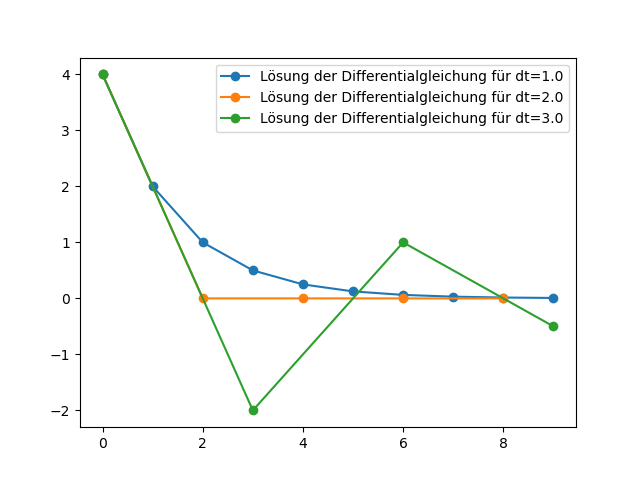
\includegraphics[width=0.7\textwidth]{media/Euler-Solutions_multiple.png}
		\caption{Das Euler-Verfahren löst eine \ac{ode} schrittweise mit konstanter Schrittweite.}
	\end{figure}
\end{frame}



